\documentclass[tikz,border=3.14mm]{standalone}
\usetikzlibrary{shapes,arrows,positioning}

\begin{document}
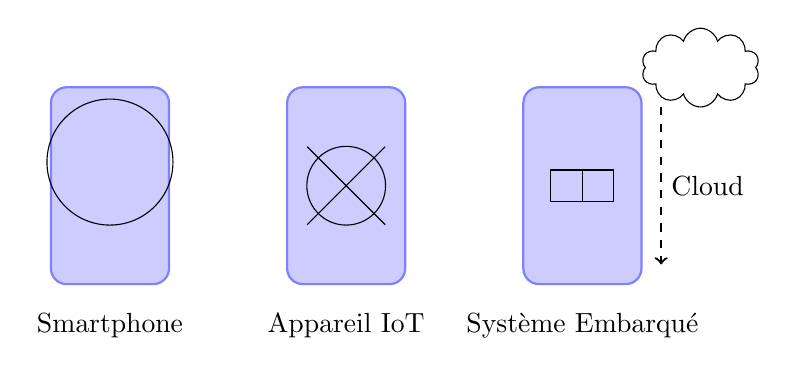
\begin{tikzpicture}[
    device/.style={rectangle, draw=blue!50, fill=blue!20, thick, minimum width=1.5cm, minimum height=2.5cm, rounded corners=0.2cm}
]

% Smartphone
\node[device] (phone) at (0,0) {};
\draw (0,0.3) circle (0.8cm);
\node[below] at (0,-1.5) {Smartphone};

% IoT device
\node[device] (iot) at (3,0) {};
\draw (3,0) circle (0.5cm);
\foreach \angle in {45,135,225,315} {
    \draw (3,0) -- ++(\angle:0.7cm);
}
\node[below] at (3,-1.5) {Appareil IoT};

% Embedded system
\node[device] (embedded) at (6,0) {};
\draw (6,-0.2) rectangle (6.4,0.2);
\draw (5.6,-0.2) rectangle (6,0.2);
\node[below] at (6,-1.5) {Système Embarqué};

% Cloud connection
\draw[->, thick, dashed] (7,1) -- (7,-1) node[midway, right] {Cloud};
\node[cloud, draw, cloud puffs=10, cloud ignores aspect, minimum width=1.5cm, minimum height=1cm] at (7.5,1.5) {};

\end{tikzpicture}
\end{document}